\documentclass[tikz,border=10mm]{standalone}
\usetikzlibrary{calc}

\def\xw{10}
\def\yw{9}
\def\rad{2.5mm}

\def\paperxw{2}
\def\paperyw{2}

\begin{document}
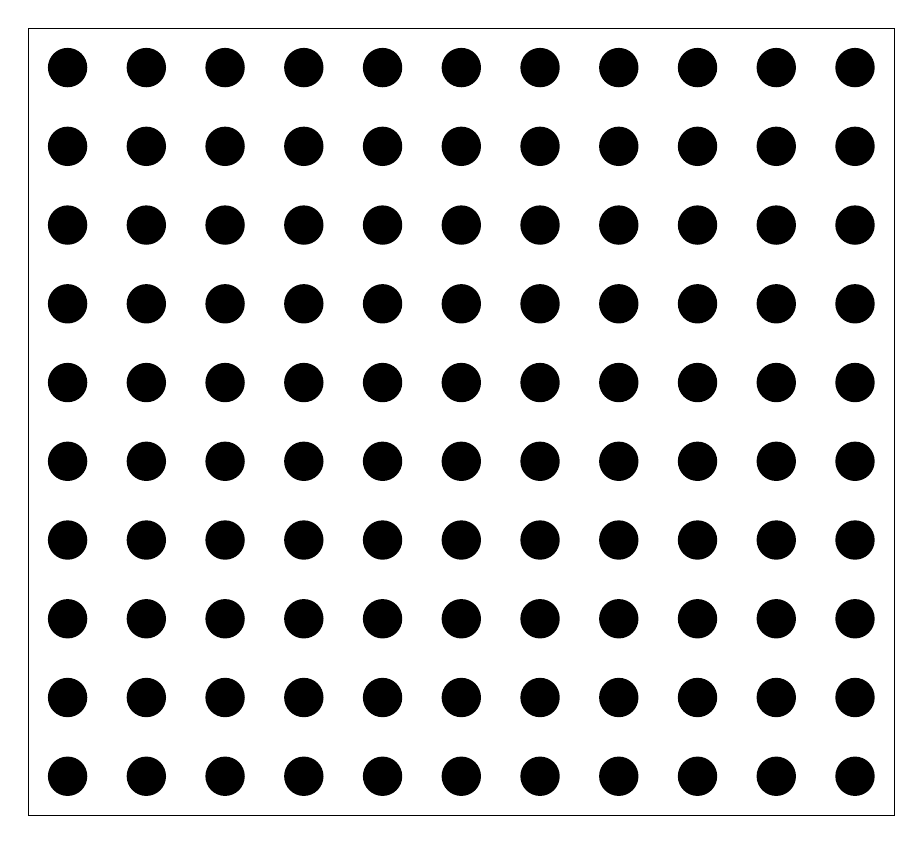
\begin{tikzpicture}[scale=1]






\draw ( 0mm ,0mm) rectangle (\xw*10.0 mm+10.0mm,\yw*10.0 mm +10.0  mm);

\foreach \b in {0,...,\xw}{
   \foreach \c in {0,...,\yw}{
      \fill[black] (\b*10.0mm+5mm,\c*10mm+5mm) circle [radius=\rad] ;
    
    }

}


\end{tikzpicture}
\end{document}
\geometry{letterpaper}
